\documentclass[11pt]{report}

%Import Packages
\usepackage{graphicx}
\usepackage{titlesec}
\usepackage{caption}
\usepackage[table]{xcolor}
%%%%%%%%%%

% Other commands
\titleformat{\chapter}{\normalfont\huge}{}{20pt}{\huge\bf}
%%%%%%%%%%


\begin{document}

\chapter{Sprint 2}

\paragraph{} In the second sprint, and our fourth week, of the project the first draft of a product backlog has been created. The main focus of the sprint will be on dividing work efforts both into working with the system development as well as on writing the report. As every other sprint, the group has the goal to be able to display a demo for the customers at the end of the sprint. 

\section{Sprint Plan} \paragraph{} As the first draft of a product backlog’s now created, the group is able to pull a number of items off the product backlog and into the sprint backlog (figure below). As most members are inexperienced in the field of web application development, and had used the previous sprint getting to know the technology better, this was the first Sprint where inexperienced started contributing to the implementation. 

\paragraph{}For cooperative programming simultaneously without causing inconsistency in the project files, the group was introduced to Git and Github by the members with previous experience with the technology. 

\begin{figure}[ht!]
\centering

\includegraphics[width=90mm]{img/Sprint2-GitnGithub.png}
\caption{Git and GitHub \label{overflow}}
\end{figure}

\paragraph{} From the beginning of the system development the back and front end development have been closely connected. For this reason, it was necessary to make sure every member was aware of how to structure the project files concerning the website. As the technical lead, Valerij briefly went through how a website usually is structurized and how we would adapt this structure to our own project. 

\paragraph{} At this stage, coding is seperated into branches and the code is tested by unit testing. Everyone working on the implementation tests their own code, with the help of others when necessary. Merging branches into the master branch on Github requires that the branches code is fully functional. When merged into the master branch integration testing will be done to make sure that the merge went smoothly and that the code of the master branch runs without errors. 

\section{Duration and Workload:}


\begin{minipage}{\linewidth}
\centering
\setlength{\tabcolsep}{22pt}
\textbf{Sprint 2:} 
\smallskip
\rowcolors{1}{blue!20}{blue!10}
\begin{tabular}{ |l l| }
	\hline
	\it{Duration} & 1 week \\
	\it{Start} & September 22nd. \\
	\it{End} & September 28th. \\
	\it{Workload} & Hours spent by the entire group on Sprint 2. \\
	\it{Goal} & 20-25 hours per person \\
	\hline
\end{tabular}
\end{minipage}

\bigskip

\begin{minipage}{\linewidth}
\setlength{\tabcolsep}{25pt}
\centering
\rowcolors{1}{blue!20}{blue!10}
\begin{tabular}{ |l|l| }
	\hline
	\multicolumn{2}{|c|}{\cellcolor{gray!25} Workload} \\
	\hline
	\it{Planning} & 20 hrs\\
	\it{Development} & 46 hrs \\
	\it{Design} & 4 hrs \\
	\it{Documentation} & 8 hrs \\
	\it{Testing} & 6.5 hrs \\
	\hline
\end{tabular}
%Caption here
\captionof{table}{Workload of Sprint 2.} 
\end{minipage}

\bigskip 

\paragraph{} The group’s goal regarding hours of work per week is 20-25 hours per person. During Sprint 2 the team did not reach their goal when it comes to working. This is further discussed in the group dynamics section a bit below. 

\section{Product Backlog}

\paragraph{} Below is the first version of the product backlog. As we were aware of the major functions required for the project, and had come quite far on developing the system requirement document, the first version of our product backlog was of some use to assign items to the Sprint 2 backlog. Unfortunately, it didn’t take long before we realized that this first version didn’t scale very well with the fast-increasing size of the backlog. 


\begin{figure}[ht!]
\centering
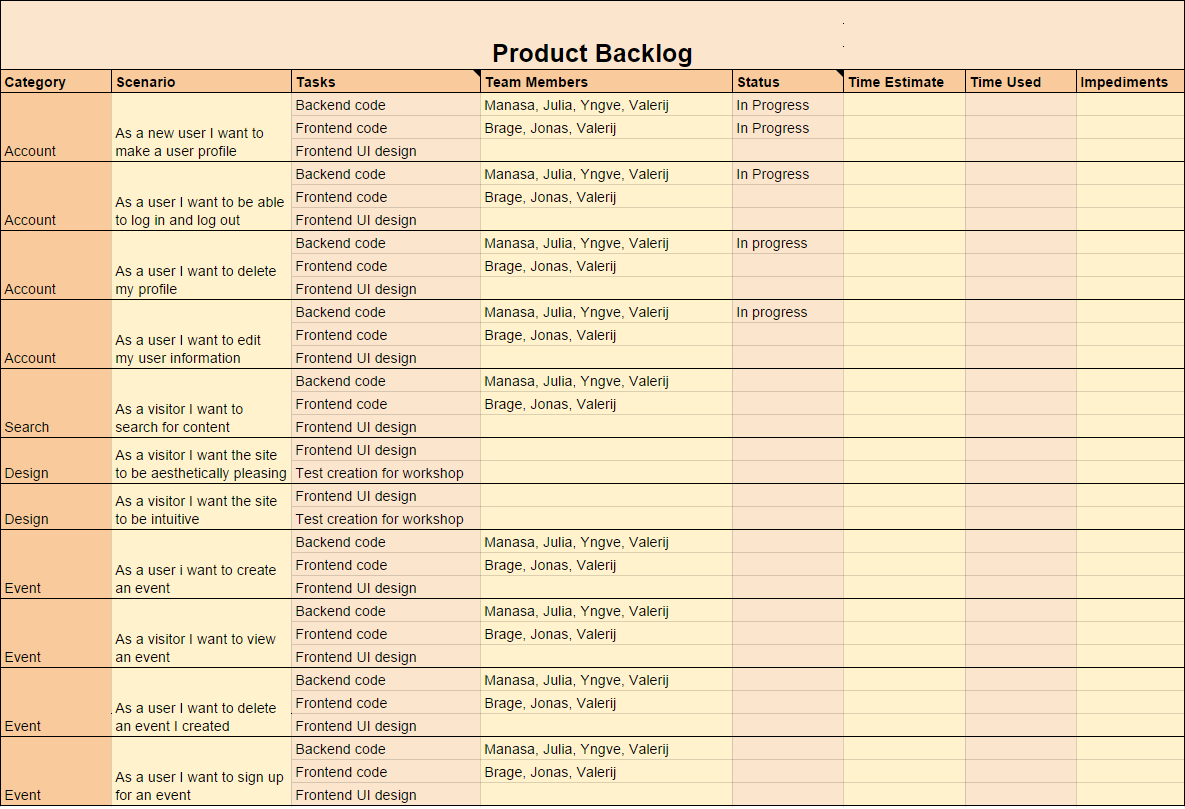
\includegraphics[width={\linewidth}]{img/Sprint2-FirstProductBacklog.png}
\caption{First Product Backlog. \label{overflow}}
\end{figure}

\section{Sprint Backlog}



\begin{minipage}{\linewidth}


\end{minipage}




\end{document}